\documentclass[10pt,notitlepage,twoside,a4paper]{scrartcl}
%
%===============================================================================================================
% packages , commands etc.
%===============================================================================================================
%\documentclass[10pt, a4paper]{scrartcl}

% fancyhdr package
%---------------------------------------------------------------------------------------------------------------
\usepackage{fancyhdr}
\pagestyle{fancy}
% with this we ensure that the chapter and section
% headings are in lowercase.
%\renewcommand{\chaptermark}[1]{%
%\markboth{#1}{}}
\renewcommand{\sectionmark}[1]{%
\markright{\thesection\ #1}}
\fancyhf{} % delete current header and footer
\fancyhead[LE,RO]{\bfseries\thepage}

% etra line for a DRAFT warning at the bottom
%\fancyfoot[CE,CO]{\textcolor{BlueViolet}{I.Sadeh \textbf{DRAFT} - \today}}

\fancyhead[LO]{\bfseries\rightmark}
\fancyhead[RE]{\bfseries\leftmark}
\renewcommand{\headrulewidth}{0.5pt}
\renewcommand{\footrulewidth}{0pt}
\addtolength{\headheight}{1.5pt} % space for the rule
\fancypagestyle{plain}{%
\fancyhead{} % get rid of headers on plain pages
\renewcommand{\headrulewidth}{0pt} % and the line
}

% in order to avoid any miss-haps when converting from dvi to pdf
\setlength{\topmargin}{0.3in}  \setlength{\headheight}{0.2in}


% included packages
%---------------------------------------------------------------------------------------------------------------
\usepackage[latin1]{inputenc}
\usepackage{amsmath}
\usepackage{amsfonts}
\usepackage{amssymb}
\usepackage{makeidx}
\usepackage[dvips,dvipsnames,usenames]{color}

% choose draft to compile without the figures
%\usepackage[draft,dvips]{graphicx}
\usepackage{graphicx}

\usepackage{varioref}

\usepackage{multirow}
\setlength{\headheight}{0in}
\usepackage{epsfig}
\usepackage{rotating}
\parskip=.1in
\usepackage{colortbl}

%\usepackage[nodayofweek]{datetime}
%\usepackage[first,light]{draftcopy}

\usepackage{mathrsfs}
% changes the shape of calligraphy fonts that are called by the command $\mathcal{A B C}$
\usepackage{eucal}
% nice calligraphy fonts: \usepackage{mathrsfs}

\usepackage{amsmath,amssymb}


% subfig and hyperref
%---------------------------------------------------------------------------------------------------------------
\usepackage{caption}
\usepackage{keyval}
\usepackage{subfig}

\newcommand{\Subref}[1]{\protect\subref{#1}}

% only a few drivers support automatically wrapped/broken links, e.g. pdftex, dvipdfm, hypertex. Other drivers lack this feature, e.g. dvips, dvipsone.   for using dvips one must place \usepackage{breakurl} after the hyperref package
\usepackage[dvips, breaklinks={true}, bookmarks, colorlinks={true}, pdfpagemode=UseNON, pdffitwindow=true, pdfstartview={FitH}, linkcolor={Blue}, menucolor={Blue}, citecolor={Red}, filecolor={OliveGreen}, urlcolor={MidnightBlue}, pdftitle={LuCaS User Guide}, pdfauthor={Bogdan Pawlik}, pdfsubject={LUCAS - UserGuide}, pdfkeywords={}]{hyperref}

\usepackage{breakurl}

\usepackage[all]{hypcap}

\labelformat{equation}{\textup{(#1)}}
\labelformat{enumi}{\textup{(#1)}}

% \Autoref is for the beginning of the sentence
\let\orgautoref\autoref
\providecommand{\Autoref}
        {\def\equationautorefname{Equation}%
         \def\figureautorefname{Figure}%
         \def\subfigureautorefname{Figure}%
         \def\sectionautorefname{Section}%
         \def\subsectionautorefname{Section}%
         \def\subsubsectionautorefname{Section}%
         \def\Itemautorefname{Item}%
         \def\tableautorefname{Table}%
         \orgautoref}

% \Autorefs is plural for the beginning of the sentence
\providecommand{\Autorefs}
        {\def\equationautorefname{Equations}%
         \def\figureautorefname{Figures}%
         \def\subfigureautorefname{Figures}%
         \def\sectionautorefname{Sections}%
         \def\subsectionautorefname{Sections}%
         \def\subsubsectionautorefname{Sections}%
         \def\Itemautorefname{Items}%
         \def\tableautorefname{Tables}%
         \orgautoref}

% \autoref is used inside a sentence 
% (this is a renew of the standard)
\renewcommand{\autoref}
        {\def\equationautorefname{Eq.}%
         \def\figureautorefname{Fig.}%
         \def\subfigureautorefname{Fig.}%
         \def\sectionautorefname{Sect.}%
         \def\subsectionautorefname{Sect.}%
         \def\subsubsectionautorefname{Sect.}%
         \def\Itemautorefname{item}%
         \def\tableautorefname{Table}%
         \orgautoref}

% \autorefs is plural for inside a sentence
\providecommand{\autorefs}
        {\def\equationautorefname{Eqs.}%
         \def\figureautorefname{Figs.}%
         \def\subfigureautorefname{Figs.}%
         \def\sectionautorefname{Sects.}%
         \def\subsectionautorefname{Sects.}%
         \def\subsubsectionautorefname{Sects.}%
         \def\Itemautorefname{items}%
         \def\tableautorefname{Tables}%
         \orgautoref}



% a footnote you can refer to multiple times
%---------------------------------------------------------------------------------------------------------------
\newcommand{\footnoteremember}[2]{

  \footnote{#2}
  \newcounter{#1}
  \setcounter{#1}{\value{footnote}}

} \newcommand{\footnoterecall}[1]{

  \footnotemark[\value{#1}]

}





% new commands
%---------------------------------------------------------------------------------------------------------------
\newcommand{\remark}[1] {\textbf{\textcolor{Mahogany}{$\rightarrow$#1$\leftarrow$}}}

\newcommand{\ps}[1] {\textcolor{OliveGreen}{ ( \underline{$\mathcal{PS}$:} \sc{#1} ) }}
%\newcommand{\ps}[1]{~}

%\newcommand{\Label}[1] {\label{#1} \textcolor{BurntOrange}{(#1)}}
%\newcommand{\Label}[1]{\label{#1}}

%\newcommand{\Cite}[1] {\cite{#1} \textcolor{blue}{(#1)}}
%\newcommand{\Cite}[1] {\cite{#1}}

\newcommand{\abs}[1] {\lvert #1 \lvert}

\newcommand{\mc}[1]{\mathcal{#1}}

% renew commands
%--------------------------------------------------------------------------------------------------------------
\renewcommand{\thefootnote}{\,\Roman{footnote}\,}
%\renewcommand{\thefootnote}{\fnsymbol{footnote}\,}


\renewcommand{\vec}[1]{\boldsymbol{#1}}

% re-set table row heigt
\renewcommand\arraystretch{1.5}

% overide the include graphics command to prevent the plots from being included
%\renewcommand\includegraphics[1][]{\textcolor{green}{filePath:~}}
%---------------------------------------------------------------------------------------------------------------


% prevent latex from EVER splitting up inline formulas.  this flag is from 1 to 10000.
% THIS CAN BE DANGEROUS !!!  :)
% rel -> penalty for splitting inline equation after relation operator
% bin -> penalty for splitting inline equation after binary operator
\relpenalty=9999
\binoppenalty=9999

%---------------------------------------------------------------------------------------------------------------

%

\date{2010-11-25}

\begin{document}
 

%\subject{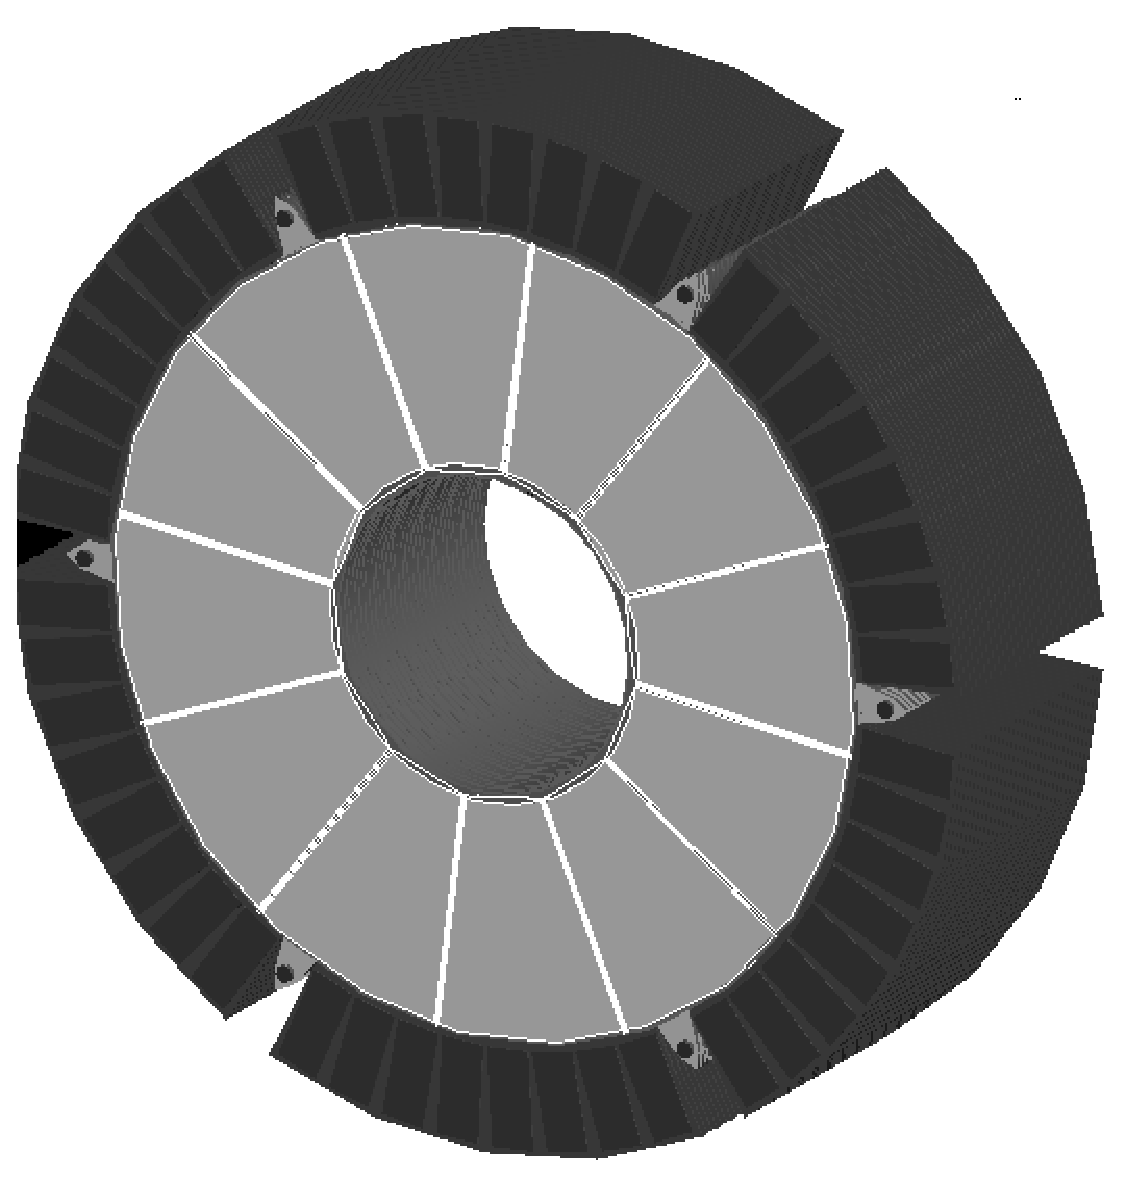
\includegraphics[bb=0 0 100 50,scale=0.2]{img/lumical}}
\subject{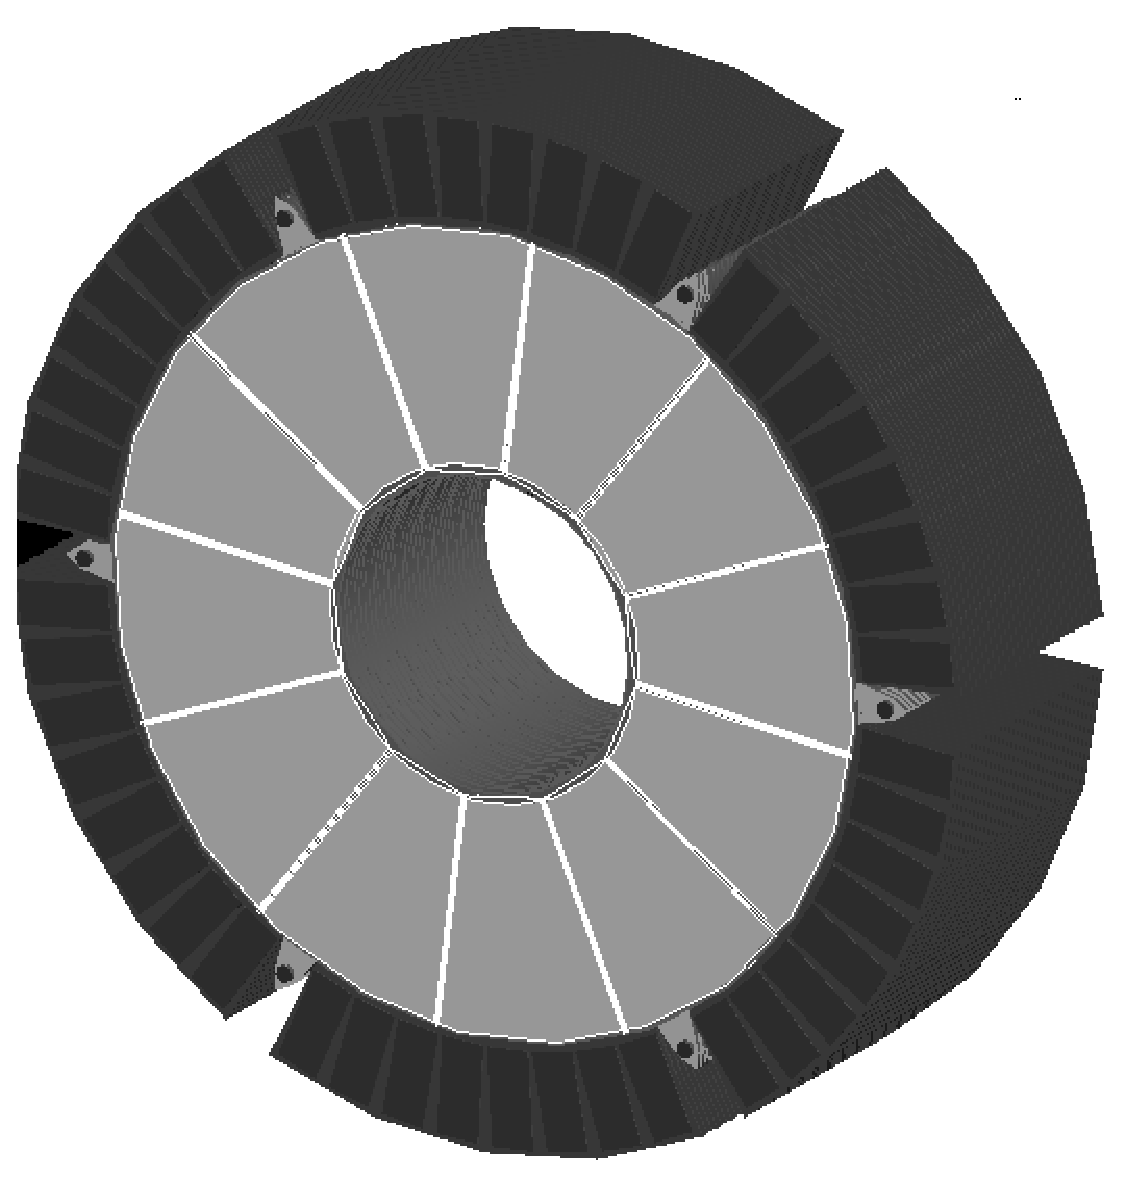
\includegraphics[scale=0.3]{img/lumical}}


\title{\Huge{\bfseries{LumiCal Simulation Package \\ User Guide}}} 

\author{\normalsize {B.~Pawlik \thanks{Institute of Nuclear Physics PAN, Cracow, Poland}}}



\maketitle \thispagestyle{empty}

% abstract
%---------------------------------------------------------------------------------------------------------------
\vspace{-30pt}
\begin{abstract}

\noindent \ps{something here ?}

\end{abstract}



 \tableofcontents
 \newpage
 \section{Introduction}
\par The LumiCal Simulation [{\bfseries LuCaS}] package is easy to use {\bf GEANT4} based application devoted for simulation of LumiCal (the luminosity monitor for ILD). Entire FCAL ( Forward Calorimetry ) detectors of ILD ( LumiCal, LHCAL, BCAL beam pipe and mask ) are build, but only LumiCal is set to be sensitive detector ({\it i.e.} hits are stored in the output file).
\newpage

 \section{Installation}\label{instal}
The LuCaS package need $Geant4$ and ROOT packages to be installed on the system.
After unpacking tarball, move to the directory LUMICAL
\begin{itemize}
 \item $>$cd LUMICAL
\end{itemize}

then inspect file setup.csh ( setup.sh if you are working with bash )
and make appropriate to your environment changes. Particulary specify location where Geant4 and ROOT
packgages are installed. Execute:
\begin{itemize}
\item $>$ source  setup.csh ( or if you are running bash  $>$. setup.sh )
\item $>$ gmake
\end{itemize}

this ( if succesfull ) will create {\bfseries{./bin/$<$OS-SYSTEM$>$}} directory where the {\bfseries{Lucas}} executable will be placed.
Now you are ready to run the program. For convinience you may want add the path to {\bfseries{Lucas}} location in to your {\bfseries PATH} environment variable.
\newpage
 \section{Using LuCaS}\label{use}
If everything went O.K. now you can start the Lucas with default confinguration in the interactive mode executing command :\\
{\bf {$>$ Lucas -i }}\\
One may want to inspect {\bf {./geant4-macros}} directory to see available visualisation macros.
 \subsection{Command line parameters}\label{params}
Full list of available command line parametrs can obtained with command:\\
{\bf {$> $Lucas -h}}\\
this will print on your screen :\\
\begin{verbatim}
Usage:          Lucas [options]


-h              print this help message and exit
-b              batch mode
-i              interactive mode (default)

-m <filename>   specifies a macro file to be executed before running
                (default none)

-o <filename>   specifies file name for ROOT output.No default
-M <mode>       specifies ROOT file opening mode ( default is NEW
                to avoid accidental file overwriting
                Possible values are RECREATE/UPDATE
-A              accumulate events from entire Run are to be
                written in one event ( suitable only for beam background data )

-c <double>     specifies the Geant 4 production range cut in mm 
                (default is 0.005 mm)
-x <double>     specifies the Beam Crossing Angle in mrad
                (default is 0 [mrad])
-s <filename>   specifies name of the file with geometry setup
-P <int>        specifies printout level ( default is 0= minimum
                                                      3= debug printout
\end{verbatim}

\newpage
 \subsection{Steering file parameters}\label{steer}

\begin{table}[http]\label{lcalpars}
\begin{center}
\begin{tabular}{lrl}
\hline
 Parameter name & Default value &  Description \\
\hline
\bf{Lcal\_z\_end}       & 2635.0 mm & defines distance of LumiCal from IP\\
\bf{Lcal\_inner\_radius}&   76.0 mm & absorber inner radius \\
\bf{Lcal\_outer\_radius}& 197.2 mm  & absorber outer radius\\
\bf{Lcal\_SensRadMin}   &  80.0 mm  & silicon sensor inner radius\\
\bf{Lcal\_SensRadMax}   & 195.2 mm  & silicon sensor outer radius\\
\bf{Lcal\_n\_layers}    &       30  & number of detector planes\\
\bf{Lcal\_n\_tiles}     &       12  & number of in one sensor plane\\
\bf{Lcal\_n\_sectors}   &       48  & number of azimuthal divisions\\
\bf{Lcal\_n\_rings}     &       64  & number of radial divisions\\
\bf{Lcal\_virtual\_cells}& 1 & virtual cells are used instead building physical one \\
& 0 & physical cells will be used\\
\end{tabular}
\caption{Full list of Lucas geometry control parameters.}
\end{center}
\end{table}
 \subsection{Accessing output tree}\label{treeacces}

\end{document}
